%\begin{titlepage}
%	
%	
%	
%	
%	% !! Basiert auf DIN A4 mit dem Font "Computer Modern" bei 11pt !!
%	\centering \singlespacing
%	
%	% Titelseitenkopf
%	\begin{minipage}{\textwidth}
%		% Logo links
%		\begin{minipage}{0.28\textwidth}
%			\centering
%			
\includegraphics[width=1\textwidth]{Figures/csgLogo.pdf} 
%		\end{minipage}
%		\hfill
%		\begin{minipage}{0.12\textwidth}	
%		\end{minipage}
%		\hfill
%		% Logo Rechts
%		\begin{minipage}{0.23\textwidth}
%			\centering
%			
\includegraphics[width=0.9\textwidth]{Figures/tu-logo.eps} %[width=1.47in]{Bilder/tu-logo.eps} 
%		\end{minipage}
%		%\hfill
%		% Fakultät und Institut rechts
%		\begin{minipage}{0.30\textwidth}
%			\large \Fakultaet \vspace{1.5mm}  \\ Institut f\"ur Energie- und  \\Automatisierungstechnik%\Institut
%		\end{minipage} %\Large
%	\end{minipage}
%	
%	% Zwischenraum
%	\vspace{4.5cm} %3cm
%	
%	% Haupt- und Untertitel 
%	{\Huge \Titel}\\[7mm]
%	\begin{minipage}{11cm}
%		\centering \LARGE   \flqq  \Untertitel \frqq
%	\end{minipage}\\
%	
%	% Zwischenraum
%	\vspace{1cm}%2.5cm
%	
%	% Gruppen- bzw. Autorenangabe
%	{\small \Gruppe}\\[0.2cm]
%	\begin{tabular}{rl}
%		\Autor  & \AutorMatrikelNr  \\
%		\ifdefempty{\AutorB}{}{\AutorB & \AutorBMatrikelNr \\} 
%		\ifdefempty{\AutorC}{}{\AutorC & \AutorCMatrikelNr \\} 
%		\ifdefempty{\AutorD}{}{\AutorD & \AutorDMatrikelNr \\} 
%		\ifdefempty{\AutorE}{}{\AutorE & \AutorEMatrikelNr \\} 
%	\end{tabular}
%	
%	% Zwischenraum
%	\vspace{3.3cm}%2cm
%	
%	% Grad
%	\begin{minipage}{11cm}
%		\centering
%		A thesis submitted for the degree of\\[0.3cm]
%		{\LARGE \textbf{-- Master of Science --}}\\[0.3cm]
%		in Computational Engineering Science
%	\end{minipage}
%	
%	
%	% 2.Zwischenraum
%	\vspace{3.3cm}
%	
%	% Professoren und Betreuer
%	\begin{tabular}{ll}
%		Examiner: & \Professor \\[1mm]
%		Co-Examiner: & \ProfessorII \\[1mm]
%		\ifdefempty{\BetreuerA}{}{Supervisor:  & \BetreuerA \\ }
%		\ifdefempty{\BetreuerB}{}{  & \BetreuerB \\ }
%	\end{tabular}
%	
%	% Umbruch bei langen Titeln verhindern
%	\enlargethispage{1cm}
%	
%	% Zwischenraum
%	\vfill
%	
%	% Footer erstellen
%	\Uni, \Fakultaet{} -- \Institut, \\ \Fachgebiet \\ \Datum
%	
%\end{titlepage}






%% !TEX encoding = UTF-8 Unicode
%% !TEX spellcheck = de_DE
%% !TEX root = ../main.tex
%
\begin{titlepage}
	\begin{spacing}{2}
			
			\begin{flushright} %rechtsbündig (Anfang)
					\vspace*{-20mm}
					
\includegraphics[width=\textwidth]{Figures/title/CoverLogos.pdf}
					%
\includegraphics[width=\textwidth]{skizzen/CoverLogos_MZH}
				\end{flushright} %rechtsbündig (Anfang)
			
			% der Titel der Arbeit:
			\vspace{38mm} {\centering {{\LARGE{\Titel}}} % Alternativ: Titel hier manuell eingeben und mit "\\"den Zeilenumbruch schön machen
					
					\vfill
					% hier kommt eine hübsche Grafik hin:
					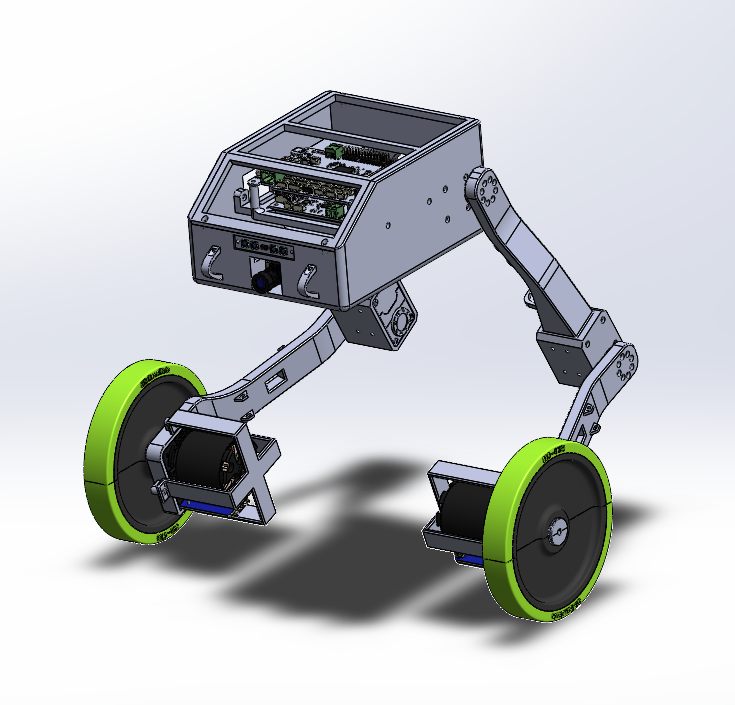
\includegraphics[width = 80mm]{Figures/title/Capture.PNG}
					
					
					\vfill }
		\end{spacing}
	\begin{spacing}{1}
			\begin{tabular}{l}
					\Large{\ArtDerArbeit~\Kennnummer}
					% Die einzutragende Nummer gibt es beim Betreuer!
				\end{tabular}
			
			\vspace{5mm}
			
			\begin{tabular}{l}
					\large{\Autor}\\
					\large{Matrikelnummer \AutorMatrikelNr}
				\end{tabular}
			
			\vspace{5mm}
			
			\begin{tabular}{l}
					\large{Hannover, \Datum}
				\end{tabular}
			
			
			\vspace{5mm}
			{\large
					\begin{tabular}{l l}						
							First Examiner  & \Erstpruefer\\
							Second Examiner & \Zweitpruefer\\
							Supervisor    	& \Betreuer\\
						\end{tabular}
				}
			
		\end{spacing}
\end{titlepage}
%\cleardoublepage